\documentclass{article}
\usepackage{iclr2027_conference,times}

\usepackage{amsmath,amssymb,amsthm}
\usepackage{booktabs}
\usepackage{graphicx}
\usepackage{microtype}
\usepackage{xcolor}
\usepackage{algorithm}
\usepackage{algpseudocode}

\newtheorem{proposition}{Proposition}
\newtheorem{lemma}{Lemma}
\newtheorem{corollary}{Corollary}
\newtheorem{remark}{Remark}

\usepackage[colorlinks=true,linkcolor=blue,citecolor=blue]{hyperref}
\usepackage{url}

\newcommand{\E}{\mathbb{E}}
\newcommand{\ind}[1]{\mathbf{1}\!\left[#1\right]}
\newcommand{\sg}{\mathrm{sg}}
\newcommand{\DensityFB}{\textsc{Density-FB}}

% Turn comments on/off:
\newif\ifcomments
\commentstrue      % show comments
%\commentsfalse     % hide comments

% Per-author comment commands
\newcommand{\aditya}[1]{%
  \ifcomments
    \textcolor{blue}{[\textbf{Aditya}: #1]}%
  \fi
}
\newcommand{\tongle}[1]{%
  \ifcomments
    \textcolor{red}{[\textbf{Tongle}: #1]}%
  \fi
}
\newcommand{\siddhant}[1]{%
  \ifcomments
    \textcolor{green}{[\textbf{Siddhant}: #1]}%
  \fi
}
\newcommand{\fan}[1]{%
  \ifcomments
    \textcolor{orange}{[\textbf{Fan}: #1]}%
  \fi
}
\newcommand{\caleb}[1]{%
  \ifcomments
    \textcolor{cyan}{[\textbf{Caleb}: #1]}%
  \fi
}
\newcommand{\benjamin}[1]{%
  \ifcomments
    \textcolor{violet}{[\textbf{Ben}: #1]}%
  \fi
}
\newcommand{\amy}[1]{%
  \ifcomments
    \textcolor{magenta}{[\textbf{Amy}: #1]}%
  \fi
}

\definecolor{fbdiff}{HTML}{2A78D6}   % lines that differ from standard FB
\definecolor{softvar}{HTML}{EB6834}  % soft-variant choice
\definecolor{hardvar}{HTML}{1A9E77}  % hard-variant choice

\title{Learning Successor Measures from Manipulation Play}
\author{%
Aditya Mohan \And Tongle Shen \And Siddhant Agarwal \And Fan Feng \\
Caleb Chuck \And Benjamin Eysenbach \And Amy Zhang
}

% \iclrfinalcopy

\begin{document}
\maketitle

% \begin{abstract}
% \caleb{not an abstract, just an outline of the intro}
% Zero shot manipulation is a highly desirable capability that FB models provide.
% However, FB models fail miserably at manipulation because of severe imprecision.
% In this work we expose the key limitation which explains this difficulty: bottleneck state misapplication of capacity
% grasping example: overly permissive when approaching the block, poor retention after grasping it
% We offer a simple and elegant solution that targets the core of this problem: Redistributing representational capacity to stabilize performance.
% by extending normalized successor-distribution learning to FB-style zero-shot control, this resolves both the core representational challenges and the zero shot control
% We show that this improves the performance of goal-conditioned benchmarks
% We also show that unseen sparse, dense and held-out rewards are possible from the same successor representation
    
% \end{abstract}

\begin{abstract}
Behavior foundation models offer the promise of zero-shot control: pretrain on offline data, then reuse learned behaviors for downstream tasks without further environment interaction.
Yet successor-measure approaches remain brittle when success depends on precise interactions.
We hypothesize that this failure arises at \emph{control bottlenecks}, where a few precise actions unlock a broad set of future behaviors, spreading their control-relevant consequences across many successor states.
We introduce \name{}, which addresses this problem by learning a normalized distribution over future states rather than regressing individual successor occupancies.
By making possible futures compete for a fixed amount of probability mass, \name{} better preserves distinctions around bottlenecks while retaining a reusable successor representation for policy learning and zero-shot reward specification.
\aditya{TODO: goal-conditioned results.}
\aditya{TODO: zero-shot transfer results.}
\end{abstract}
    
% Successor measures are a compelling route to BFMs, but cstruggle with precision.
Behavior foundation models (BFMs) offer the tantalizing promise of creating generally capable agents: simply pretrain policies using offline data that offers broad coverage, and recover optimal policies for a wide range of tasks~\citep{pirotta-iclr24a,sikchi-arxiv25a,li-iclr26a}.
For example, such pretraining can enable a robot to perform complex manipulations, even those not exactly demonstrated in the dataset. 
Successor-measure (SM) methods provide a natural framework for this goal.
Methods such as Forward-Backward representations (FB)~\citep{touati-neurips21a,touati-iclr23a} and Proto-Successor Measures (PSM)~\citep{agarwal-icml25a} learn reusable representations that, in principle, support zero-shot policy recovery for rewards that were never specified during pretraining.
Yet this promise remains difficult to realize when control requires precise interactions~\citep{cetin-rlj24a,mohan-rlbrew26a}.
In manipulation, FB can reach the relevant object while failing at the interaction that determines task success, such as establishing a reliable grasp in cube pick-and-place, causing performance to deteriorate sharply as tasks require more precise or compositional behavior~\citep{mohan-rlbrew26a}.

% Our hypothesis: control bottlenecks expose a weakness of successor-density approximation:
We hypothesize that this loss of precision arises at \emph{control bottlenecks}: states where a small number of precise actions determine access to a much broader region of future behavior.
Unlike classical TD learning, which compresses an action's consequences into a scalar value for a given reward, SM methods must represent the full distribution of possible future states.
This distinction becomes particularly important at a bottleneck, where the effect of a critical action may only become apparent across the large set of states that become reachable afterwards.
Consider the state immediately before grasping a cube. 
For many nearby future states, successful and unsuccessful grasping actions induce similar successor predictions because the cube has not yet moved.
The distinction that matters for control appears primarily after the bottleneck: a successful grasp makes a large family of downstream cube configurations reachable, whereas a failed grasp does not. 
This action-discriminative signal is therefore distributed across many individual future states. 
Under finite-capacity SM-approximation, the model must simultaneously represent the large set of weakly informative futures and this diffuse but control-critical downstream region, potentially allocating insufficient capacity to the latter.
This mismatch explains why SM models can accurately capture coarse future occupancy while still failing at the precise interactions that determine task success. 
The same structure arises beyond manipulation: passing through a narrow doorway can unlock an entire region in navigation, placing a foot correctly can determine access to subsequent locomotion states, and picking up a key or opening a door can make a large set of otherwise unreachable states accessible.

% This means that the learned successor model fails to sufficiently allocate representational capacity to the precision-sensitive components (ex. the initial grasp in manipulation). Intuitively, this is because instead of learning to represent a single number, as with classical TD learning, SM models must capture a full distribution of possible futures. For example, consider again the block picking example. Suppose we approximate the successor measure of a state and action before the grasp, and compare what happens based on which future state we sample. For a future state sampled before the bottleneck state, any action that is taken has little effect on the outcome of the bottleneck---the block stays in the same position. If sampled after the bottleneck state, the representational capacity is diffused over the full space of possibilities for the block. This significant mismatch between the two representations results tangibly in poor optimization and final performance. However, this property is not manipulation specific, but plagues any environment where a policy is missing a future state.

% We changes the approximation geometry by modeling the normalized successor distribution
In this work, we provide a simple, elegant solution to this problem: rather than learning each future-state occupancy in isolation, we let possible futures compete for a fixed amount of successor probability. 
Our method, \name{}, recasts the successor measure as a normalized distribution over future states and extends it to FB-style zero-shot control. 
Normalization preserves the information in the successor measure while changing what the model must learn: instead of matching the absolute magnitude of individual occupancy values, it must determine how to allocate future probability across competing outcomes.
We then train this distribution directly with a cross-entropy Bellman objective, so errors correspond to placing too much probability on some futures and too little on others. At a control bottleneck, this means that a successful action is rewarded for shifting probability mass toward the entire downstream region it unlocks, rather than requiring each of those future states to carry a strong learning signal on its own. \name{} therefore makes the consequences of precise bottleneck actions easier to distinguish while retaining the reusable successor representation central to FB.

% Concretely, \name{} utilizes the FB bilinear product as a log-density score and replaces squared successor-density regression with a cross-entropy Bellman objective over the normalized distribution, thereby re-balancing how SM approximation allocates capacity across possible futures. 
% This changes the relative importance of approximation errors across future states, reducing the dominance of concentrated successor regions and better preserving collectively important distinctions across diffuse post-bottleneck futures. Density-FB thereby retains the reusable successor representation central to FB while making it better suited to precision-sensitive control.


% Old
% In this work, we provide a simple, elegant solution to this problem by rebalancing the representational capacity: apply self-normalizing weights to the successor measure values, then replace the objective with a cross-entropy one. This is inspired by two insights. First, normalizing the successor measure estimate balances the overestimation bias from the "before bottleneck" sampling with the underestimation of the "after bottleneck" sampling. Second, both these elements, but especially the cross-entropy objective, stabilizes the learning process, preventing the successor measure values to become extreme, and then unusable. By extending normalized successor-distribution learning to FB-style zero-shot control, this resolves both the core representational challenges and enables zero shot control in manipulation environments. Combined, these modifications make FB more robust to bottleneck states, especially when training with a neural network.

% Evidence: What are we able to demonstrate and why is that important

% COntributions: Our list of contributions in paraenum

\aditya{
TODO: flesh this out with results.
We show that this improves the performance of goal-conditioned benchmarks
We also show that unseen sparse, dense and held-out rewards are possible from the same successor representation
}



% Zero shot manipulation is a highly desirable capability that FB models provide.
% However, FB models fail miserably at manipulation because of severe imprecision.
% In this work we expose the key limitation which explains this difficulty: bottleneck state misapplication of capacity
% grasping example: overly permissive when approaching the block, poor retention after grasping it
% We offer a simple and elegant solution that targets the core of this problem: Redistributing representational capacity to stabilize performance.
% by extending normalized successor-distribution learning to FB-style zero-shot control, this resolves both the core representational challenges and the zero shot control
% We show that this improves the performance of goal-conditioned benchmarks
% We also show that unseen sparse, dense and held-out rewards are possible from the same successor representation


\section{Preliminaries}
\label{sec:prelim}

\paragraph{Offline reward-free setting.}
We consider a discounted Markov decision process $\mathcal M=(\mathcal S,\mathcal A,P,\gamma)$ with $\gamma\in(0,1)$. 
The agent is given a fixed dataset $\mathcal D=\{(s_i,a_i,s_i')\}_{i=1}^{N}$ collected without downstream reward labels.
We denote by $\rho$ the marginal distribution of next states $s'$ in $\mathcal D$. 
Downstream tasks are specified by rewards $r:\mathcal S\rightarrow\mathbb R$.

\paragraph{Successor measures.}
For a policy $\pi$, define its discounted successor measure over future states as
\begin{equation}
    M^\pi(s,a,X) := \E_\pi\!\left[ \sum_{t\ge0}\gamma^t \ind{s_{t+1}\in X} \;\middle|\; s_0=s,\;a_0=a \right],
    \label{eq:sm}
\end{equation}
for measurable $X\subseteq\mathcal S$.
It satisfies the Bellman recursion
\begin{equation}
    M^\pi(s,a,\cdot) = P(\cdot\mid s,a) + \gamma \E_{\substack{ s'\sim P(\cdot\mid s,a)\\ a'\sim\pi(\cdot\mid s')}} \left[ M^\pi(s',a',\cdot) \right].
    \label{eq:sm-bellman}
\end{equation}
For any downstream reward $r$, integrating $r$ against the successor measure recovers its action value,
\begin{equation}
    Q_r^\pi(s,a) = \int_{\mathcal S} r(s^+)\,M^\pi(s,a,ds^+) = \E_\pi\!\left[ \sum_{t\ge0}\gamma^t r(s_{t+1}) \;\middle|\; s_0=s,\;a_0=a \right].
    \label{eq:sm-value}
\end{equation}
Importantly, every successor measure has fixed total mass
\begin{equation}
    M^\pi(s,a,\mathcal S) = \sum_{t\ge0}\gamma^t = \frac{1}{1-\gamma}.
    \label{eq:sm-mass}
\end{equation}
\section{\name{}}
\label{sec:method}

\name{} replaces FB's regression of an unnormalized successor measure with categorical learning of its normalized distribution. We derive the resulting Bellman objective and show how the learned distribution supports policy learning and downstream reward specification.
Algorithm~\ref{alg:dfb} summarizes \name{} training and zero-shot deployment.

\subsection{Learning normalized successor distributions}
\label{sec:method-density}

Since $M^\pi(s,a,\mathcal S)=1/(1-\gamma)$, we define the normalized successor measure as $\nu^\pi(s,a,\cdot):=(1-\gamma)M^\pi(s,a,\cdot)$. 
It is a probability measure over future states, and Equation~\eqref{eq:sm-bellman} gives the Bellman recursion
\begin{equation}
    \nu^\pi(s,a,\cdot) = (1-\gamma)P(\cdot\mid s,a) + \gamma\E_{\substack{s'\sim P(\cdot\mid s,a)\\a'\sim\pi(\cdot\mid s')}}\left[\nu^\pi(s',a',\cdot)\right].
    \label{eq:normalized-bellman}
\end{equation}
Thus, $1-\gamma$ of the successor probability comes from the immediate transition, while the remaining $\gamma$ is propagated from subsequent states.

For the policy indexed by $z$, let
\[
    h_z(s,a,s^+) := \frac{d\nu^{\pi_z}(s,a,\cdot)}{d\rho}(s^+)
\]
denote its normalized successor-density ratio. 
Whereas standard FB directly approximates the density of the unnormalized successor measure with a bilinear factorization, \name{} uses the same factorization as a log-density score,
\begin{equation}
    f_\theta(s,a,z,s^+) := \frac{F_\theta(s,a,z)^\top B_\theta(s^+)}{\tau}, \qquad h_\theta(s,a,z,s^+) := \frac{\exp f_\theta(s,a,z,s^+)}{\E_{\tilde s^+\sim\rho}\left[\exp f_\theta(s,a,z,\tilde s^+)\right]}.
    \label{eq:density-model}
\end{equation}
Hence $F_\theta^\top B_\theta/\tau$ is a log-density score, while its normalized exponential models the successor-density ratio $h_z$.

We approximate the normalization in Equation~\eqref{eq:density-model} using the next states in a minibatch as samples from $\rho$. 
For $\{(s_i,a_i,s_i')\}_{i=1}^{n}$, define
\begin{equation}
    p_{ij} := \operatorname{softmax}_{j}\left(f_\theta(s_i,a_i,z_i,s_j')\right).
    \label{eq:density-softmax}
\end{equation}
Each row $p_i$ is a categorical distribution over the empirical candidate states $\{s_j'\}_{j=1}^{n}$.

To construct its Bellman target, let $a_i'=\sg[\pi_\omega(s_i',z_i)]$ and define the target-network prediction
\begin{equation}
    \bar p_{ij}' := \operatorname{softmax}_{j}\left(\frac{\bar F(s_i',a_i',z_i)^\top\bar B(s_j')}{\tau}\right).
    \label{eq:target-density-softmax}
\end{equation}
Equation~\eqref{eq:normalized-bellman} then yields the categorical Bellman target
\begin{equation}
    p_{ij}^{\mathrm{tgt}} := \sg\left[(1-\gamma)\mathbf 1[j=i]+\gamma\bar p_{ij}'\right].
    \label{eq:bellman-target}
\end{equation}
We fit the predicted distribution with cross-entropy,
\begin{equation}
    \mathcal L_{\mathrm{occ}} := -\frac{1}{n}\sum_{i=1}^{n}\sum_{j=1}^{n}p_{ij}^{\mathrm{tgt}}\log p_{ij}.
    \label{eq:occupancy-loss}
\end{equation}
This update parallels the categorical Bellman update in TD-InfoNCE~\citep{zheng-iclr24a}; here, we use it to learn the $z$-conditioned family of successor distributions required for FB-style control.

\subsection{Policy learning from successor distributions}
\label{sec:method-control}

A normalized successor density determines the value of any state-based reward by integration. 
For a policy $\pi_z$, define
\begin{equation}
    q_r^{\pi_z}(s,a) := \E_{s^+\sim\rho}\left[h_z(s,a,s^+)r(s^+)\right] = (1-\gamma)Q_r^{\pi_z}(s,a).
    \label{eq:normalized-value}
\end{equation}
\name{} estimates this quantity by replacing the true density ratio with the learned model,
\begin{equation}
    q_{\theta,r}(s,a,z) := \E_{s^+\sim\rho}\left[h_\theta(s,a,z,s^+)r(s^+)\right].
    \label{eq:reward-readout-population}
\end{equation}
For a finite candidate pool $\{s_j^+\}_{j=1}^{P}$, we use
\begin{equation}
    q_{\theta,r}(s,a,z) \approx \sum_{j=1}^{P}p_j(s,a,z)r(s_j^+), \qquad p_j(s,a,z):=\operatorname{softmax}_{j}\left(f_\theta(s,a,z,s_j^+)\right).
    \label{eq:reward-readout}
\end{equation}
Thus, rather than reading value directly from $F(s,a,z)^\top z$ as in standard FB, \name{} evaluates an action by integrating the requested reward under its predicted successor distribution.

During pretraining, each task index $z$ is paired with a reward $r_z$. 
In the goal-conditioned setting, for example, $z=g$ and $r_g$ rewards reaching the sampled goal. 
Let $\hat q_{s,z}:=q_{\theta,r_z}(s,\pi_\omega(s,z),z)$. We train a behavior-regularized actor with
\begin{equation}
    \mathcal L_{\pi} := -\frac{\E_{s,z}\left[\hat q_{s,z}\right]}{\sg\left[\E_{s,z}\left|\hat q_{s,z}-\E[\hat q_{s,z}]\right|+\varepsilon\right]}+\beta\mathcal L_{\mathrm{BC}}(\pi_\omega).
    \label{eq:actor-loss}
\end{equation}
The normalization controls the scale of the value term relative to behavior cloning. 
During the actor update, gradients are propagated through the action input to $F_\theta$.

\subsection{Zero-shot reward specification}
\label{sec:method-task-interface}

Standard FB obtains a downstream task vector from the linear identity
\begin{equation}
    \int_{\mathcal S} r(s^+)F(s,a,z)^\top B(s^+)\,d\rho(s^+) = F(s,a,z)^\top\E_\rho[r(s^+)B(s^+)],
    \label{eq:fb-linear-identity}
\end{equation}
which yields the closed-form reward embedding $z_r\propto\E_\rho[rB]$.
\name{} does not preserve this identity because $F^\top B$ now parameterizes a log-density score rather than the successor density itself.
The standard FB reward embedding is consequently not a well-defined task interface for the normalized model; Appendix~\ref{app:fb-task-map} gives the
corresponding invariance argument.

Instead, we infer the downstream task directly in the pretrained policy space. 
For an unseen reward $r$, define
\begin{equation}
    J_{\theta,r}(z) := \E_{s\sim\mu_{\mathrm{sel}}} \left[ q_{\theta,r}(s,\pi_\omega(s,z),z) \right], \qquad z_r^\star \in \arg\max_{z\in\mathcal Z} J_{\theta,r}(z).
    \label{eq:policy-search}
\end{equation}
Once a family of policies is learned offline, downstream objectives can be optimized directly over its low-dimensional task index without additional environment interaction or parameter updates.

\begin{algorithm}[t]
\caption{\name{}}
\label{alg:dfb}
\begin{algorithmic}[1]
\Require Offline dataset $\mathcal D$, successor model $F_\theta,B_\theta$, target models $\bar F,\bar B$, actor $\pi_\omega$, discount $\gamma$, temperature $\tau$, BC coefficient $\beta$
\For{each training iteration}
    \State Sample transitions $\{(s_i,a_i,s_i')\}_{i=1}^{n}\sim\mathcal D$
    \State Sample task/reward pairs $\{(z_i,r_{z_i})\}_{i=1}^{n}$
    \State Compute successor probabilities $p_{ij}$ using Equation~\eqref{eq:density-softmax}
    \State $a_i'\gets\sg[\pi_\omega(s_i',z_i)]$
    \State Compute target probabilities $\bar p_{ij}'$ using Equation~\eqref{eq:target-density-softmax}
    \State $p_{ij}^{\mathrm{tgt}}\gets\sg[(1-\gamma)\mathbf 1[j=i]+\gamma\bar p_{ij}']$
    \State Update $F_\theta,B_\theta$ by minimizing $\mathcal L_{\mathrm{occ}}$ in Equation~\eqref{eq:occupancy-loss}
    \State Estimate $q_{\theta,r_{z_i}}(s_i,\pi_\omega(s_i,z_i),z_i)$ using Equation~\eqref{eq:reward-readout}
    \State Update $\pi_\omega$ by minimizing $\mathcal L_\pi$ in Equation~\eqref{eq:actor-loss}
    \State Update $\bar F,\bar B$ by exponential moving average
\EndFor
\Statex
\Statex \textbf{Zero-shot deployment}
\State Given downstream reward $r$, select $\hat z_r$ from $\mathcal Z_{\mathrm{cand}}$ using Equation~\eqref{eq:policy-search}
\State Execute the frozen policy $\pi_\omega(\cdot,\hat z_r)$
\end{algorithmic}
\end{algorithm}
% % ======================================================================
\section{Goal-conditioned results}
\label{sec:main-results}

We evaluate on state-based OGBench manipulation and locomotion
\citep{park2024ogbench}.
All of our models are trained for $500$k gradient steps with no reward labels.
Native evaluation uses five tasks, $50$ episodes each, and three seeds; intervals are $95\%$ $t$-based confidence intervals.

We evaluate each representation with two actor extractors, FQL + BC and Gaussian DDPG+BC, to separate representation quality from policy extraction.
Behavior cloning trains the same actor with the $q_g$ term removed and learns no successor representation: it reaches $0.111$ on \texttt{cube-single} and $0.019$ on \texttt{cube-double}.
Published GCIQL results use $1$M gradient steps and eight seeds.
We include them as an external reference rather than a matched baseline.

\begin{table}[h]
\centering
\small
\setlength{\tabcolsep}{3pt}
\begin{tabular}{llcccc}
\toprule
Environment & Actor & Plain FB & \DensityFB{} (soft) & \DensityFB{} (hard) & \shortstack{GC-IQL\\(published)} \\
\midrule
\texttt{cube-single}
& FQL + BC
& $0.420$
& $\mathbf{0.929 \pm 0.085}$
& $0.915 \pm 0.087$
& -- \\

& DDPG + BC
& $0.353 \pm 0.38$
& $0.879 \pm 0.095$
& $0.887 \pm 0.066$
& $0.68 \pm 0.06$ \\
\midrule

\texttt{cube-double}
& FQL + BC
& $0.005 \pm 0.016$
& $\mathbf{0.736 \pm 0.139}$
& $0.680 \pm 0.070$
& -- \\

& DDPG + BC
& $0.013 \pm 0.029$
& $\mathbf{0.646 \pm 0.019}$
& $0.599 \pm 0.077$
& $0.40 \pm 0.05$ \\
\midrule

\texttt{scene}
& FQL + BC
& $0.076 \pm 0.057$
& $0.628 \pm 0.134$
& $\mathbf{0.641 \pm 0.109}$
& -- \\

& DDPG + BC
& $0.047 \pm 0.057$
& $0.563 \pm 0.011$
& $0.581 \pm 0.322$
& $0.51 \pm 0.04$ \\
\midrule

\texttt{antmaze-medium}
& FQL + BC
& $0.593 \pm 0.25$
& $0.563 \pm 0.167$
& $0.669 \pm 0.240$
& -- \\

& DDPG + BC
& \emph{pending}
& $0.829 \pm 0.058$
& $\mathbf{0.877 \pm 0.097}$
& $0.71 \pm 0.04$ \\
\bottomrule
\end{tabular}

\caption{
Native goal-conditioned success by environment and policy-extraction rule.
All \DensityFB{} cells use three seeds except \texttt{cube-double} with DDPG + BC, which uses four. Plain FB uses three seeds except \texttt{cube-double} with FQL + BC (four) and \texttt{scene} with FQL + BC (five). The \emph{pending} cell never ran: its launch failed because the AntMaze dataset was absent from the expected path.
Seeds for the completed manipulation cells:
soft flow \texttt{cube-single} $.896/.928/.964$,
\texttt{cube-double} $.680/.736/.792$,
\texttt{scene} $.672/.568/.644$;
hard flow \texttt{cube-single} $.876/.944/.924$,
\texttt{cube-double} $.692/.700/.648$,
\texttt{scene} $.692/.620/.612$;
soft DDPG + BC \texttt{cube-double} $.644/.660/.648/.632$,
hard DDPG + BC \texttt{cube-double} $.668/.560/.596/.572$.
}
\label{tab:main}
\end{table}

On \texttt{cube-single}, both \DensityFB{} variants reach about $0.92$, leaving little room to distinguish them.
The harder manipulation tasks separate the methods more clearly.
On \texttt{cube-double}, soft \DensityFB{} reaches $0.736$ with the flow actor, compared with $0.005$ for plain FB and $0.019$ for behavior cloning; with DDPG+BC it reaches $0.646$, against a published $0.40$ for GCIQL at twice the training budget.
On \texttt{scene}, \DensityFB{} reaches about $0.64$ while plain FB remains near zero.

The \texttt{scene} average also hides a consistent task split.
All seeds solve \texttt{open}, \texttt{unlock-and-lock}, and \texttt{rearrange-medium} ($0.88$--$1.0$).
\texttt{put-in-drawer} ($0.02$--$0.50$) and \texttt{rearrange-hard} ($0.0$--$0.04$) remain difficult.

\paragraph{Manipulation results are similar under DDPG+BC.}
Switching from FQL + BC to DDPG+BC lowers soft \DensityFB{} from $0.929$ to $0.879$ on \texttt{cube-single} and from $0.736$ to $0.646$ on \texttt{cube-double}.
The improvement is therefore not specific to the flow actor.
On \texttt{antmaze-medium}, the same switch moves \DensityFB{} from $0.563$ to $0.829$, so actor extraction matters much more there.

\paragraph{\DensityFB{} does not improve AntMaze.}
\texttt{antmaze-medium} removes the structure that motivated \DensityFB{}: the goal-relevant variable is the agent itself, so there is no manipulated object that remains stationary while actions continue.
Under DDPG+BC, \DensityFB{} reaches $0.829$ against $0.837$ for our matched GCIQL control, and both remain below the strongest published method on that benchmark ($0.96$ for HIQL).
This supports the narrower hypothesis that \DensityFB{} helps when play data contains long stationary segments in the goal-relevant object variables.

\paragraph{Isolating the estimator from the outcome coordinates.}
\DensityFB{} departs from FB in two places at once: the categorical estimator, and the privileged outcome coordinates $\phi$ that the successor measure is predicted over.
Two controls separate them on \texttt{cube-double}, the discriminating environment, matched in everything else (one seed each, $500$k steps; we quote the $500$k value and, in parentheses, the mean over evaluations after $350$k).
A paper-exact TD InfoNCE critic (Proposition~\ref{prop:tdinfonce}) reaches $0.576$ ($0.545$).
A goal-conditioned outcome-space LSIF model --- FB's own unnormalized loss, but on our $\phi$, with our external kernel readout and our actor --- reaches $0.300$ ($0.329$).
Both fall below soft \DensityFB{} ($0.736$) and hard \DensityFB{} ($0.680$).
Read together they split the improvement: $\phi$ plus an external readout carries plain FB from $0.005$ to $0.300$, and the normalized categorical estimator carries $0.300$ to $0.736$.
The privileged coordinates are therefore load-bearing, and the estimator change still accounts for the larger share.
These are single-seed runs, and the matched-extractor TD InfoNCE arm has not been run (Section~\ref{sec:todo}).

% ======================================================================
\section{Reward evaluation}
\label{sec:reward-transfer}

Goal reaching only tests whether the learned measure supports the benchmark goals.
Reward transfer asks whether the same measure can evaluate a reward that was never used for training.

At test time, we draw a pool $U_P=\{u_j\}_{j=1}^{16{,}384}$ of object configurations from the dataset.
For a given $(s,a,g)$, we compute the normalized occupancy $p(s,a,g;U_P)$ over this pool and evaluate the reward once on every pool element.
The direct Monte-Carlo readout is
\begin{equation}
    \frac{ p(s,a,g;U_P)^\top r(U_P) }{ 1-\gamma}.
\end{equation}

Because stationary transitions concentrate predicted occupancy near the current object configuration, finite-pool smoothing matters most there.
We therefore apply a local correction at $x=\phi(s).$

Let $ c_x\in\Delta^{|U_P|-1}$ denote the normalized kernel weights of $x$ over the pool (the same $k^\epsilon$ as Equation~\ref{eq:goal-readout}).
We replace the interpolated reward $c_x^\top r(U_P)$ with its exact value $r(x)$:
\begin{equation}
\label{eq:density-readout}
    \widehat Q_r(s,a,g) = \frac{ r(x) + \left( p(s,a,g;U_P)-c_x \right)^\top r(U_P)}{1-\gamma}.
\end{equation}
The correction is action independent, so it changes the absolute value estimate without changing the ranking of actions.
The resulting readout remains linear in $r$ and requires no retraining.

To act under a new reward, we score candidate goals using Equation~\ref{eq:density-readout}, select the highest-valued goal from the initial state, and execute its goal-conditioned policy.
This replaces FB's analytic reward-to-$z$ mapping with search over the learned goal-conditioned policy family.

\paragraph{Reward construction.}
We test three reward families, all defined only from object coordinates, valued in $[0,1]$, and never observed during training (Figure~\ref{fig:rewardfams}; internal names \texttt{dirac}/\texttt{dense}/\texttt{region}):

\emph{sparse}, the benchmark tolerance indicator
\begin{equation}
    r(x) = \ind{\|x-g\|\le\epsilon},
\end{equation}
conjunctive over object blocks, at the five task goals;

\emph{dense}, the same centers with distance-based shaping
\begin{equation}
    r(x) = \exp(-d(x,g)/2\epsilon)
\end{equation}
in tolerance-scaled coordinates;
and \emph{held-out regions}, the same sparse indicator centered at reachable dataset configurations that are not benchmark goals.
These centers are drawn by hindsight from within episodes and kept only when at least five relabeled samples fall inside the region.
Dense versus sparse varies reward shaping while keeping the goal fixed.
Sparse versus held-out regions keeps the reward form fixed while changing where in object space the reward is located.
We evaluate $25$ episodes per task and three seeds.
The fixed-partition ablation replaces the resampled query set with $256$ fixed prototypes while leaving the rest of the objective unchanged.

\begin{figure}[t]
\centering
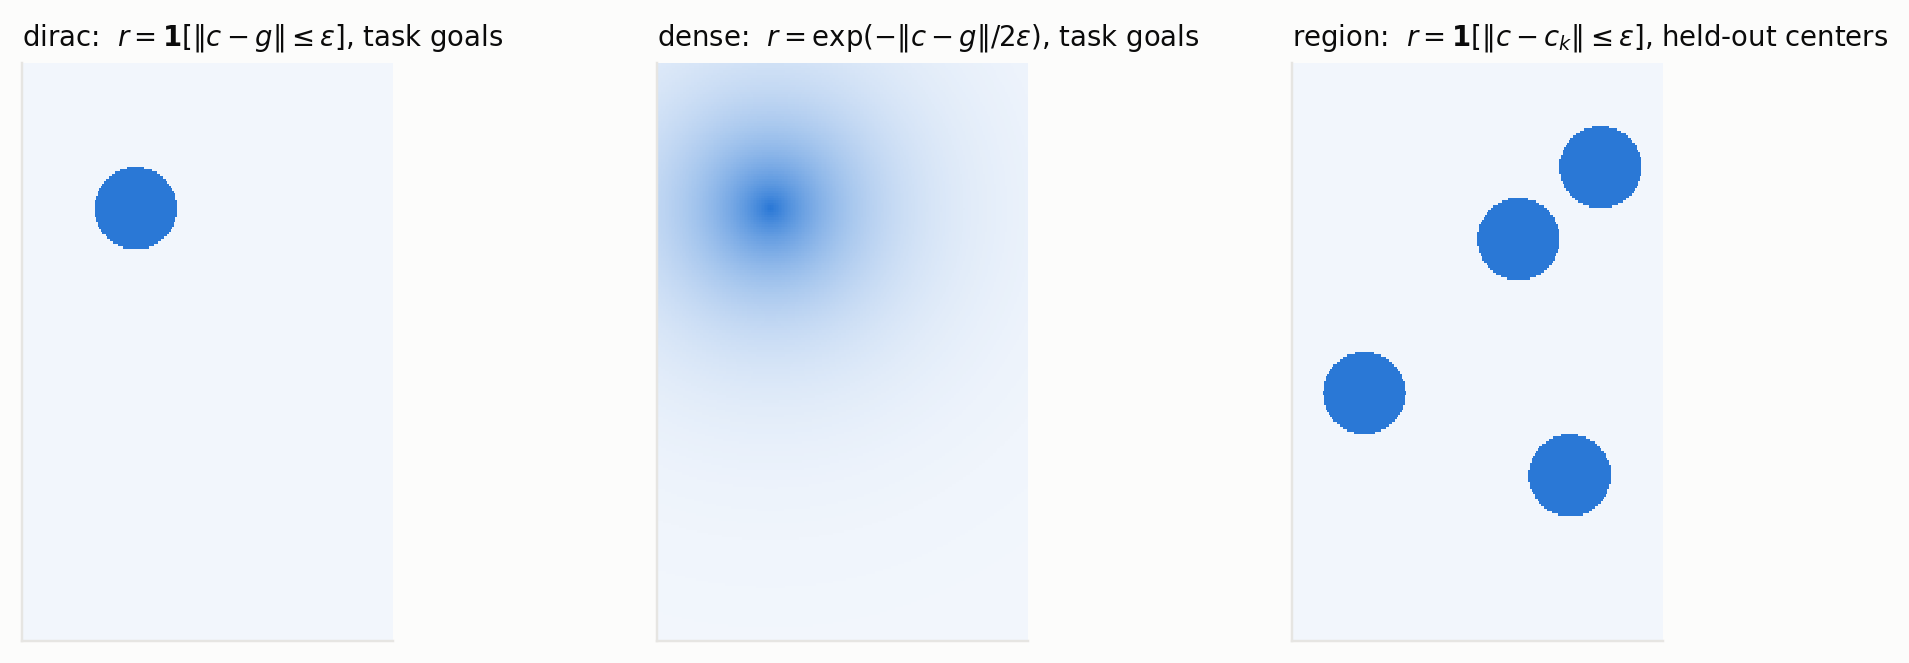
\includegraphics[width=0.95\textwidth]{figures/reward-families.png}
\caption{
The three test reward families on the cube workspace
(cube-position plane, $\epsilon$-balls to scale).
Sparse and dense share task-style centers and differ in shaping;
held-out regions keep the sparse form at hindsight-drawn dataset centers.
}
\label{fig:rewardfams}
\end{figure}

\begin{table}[h]
\centering
\small
\setlength{\tabcolsep}{4pt}
\begin{tabular}{llccc}
\toprule
Environment & Reward family & Plain FB & \DensityFB{} (soft) & \DensityFB{} (hard) \\
\midrule

\texttt{cube-single}
& sparse
& $0.413 \pm 0.308$
& $0.816 \pm 0.269$
& $\mathbf{0.888 \pm 0.091}$ \\

& dense
& $0.488 \pm 0.397$
& $0.725 \pm 0.301$
& $\mathbf{0.912 \pm 0.087}$ \\

& held-out regions
& $0.090 \pm 0.114$
& $0.293 \pm 0.052$
& $\mathbf{0.647 \pm 0.301}$ \\
\midrule

\texttt{cube-double}
& sparse
& $0.013 \pm 0.023$
& $0.549 \pm 0.240$
& $\mathbf{0.573 \pm 0.126}$ \\

& dense
& $0.037 \pm 0.011$
& $0.488 \pm 0.163$
& $\mathbf{0.520 \pm 0.121}$ \\

& held-out regions
& $0.000 \pm 0.000$
& $0.177 \pm 0.160$
& $0.167 \pm 0.014$ \\
\midrule

\texttt{scene}
& sparse
& $0.472 \pm 0.124$
& $0.395 \pm 0.092$
& $\mathbf{0.640 \pm 0.111}$ \\

& dense
& $0.413 \pm 0.030$
& $0.347 \pm 0.219$
& $\mathbf{0.627 \pm 0.094}$ \\

& held-out regions
& $0.053 \pm 0.080$
& $0.220 \pm 0.086$
& $\mathbf{0.347 \pm 0.038}$ \\
\bottomrule
\end{tabular}

\caption{
Zero-shot reward transfer
(mean $\pm$ $95\%$ CI, three seeds unless marked).
GCIQL has no reward readout of this kind and is therefore absent.
Plain FB is evaluated through its own reward interface, $z_r \propto \E_\rho[r(x)B(x)]$ followed by rollout under $z_r$, since it has no density readout; the reward families, pool, episode count, and success criterion are identical across all three columns, so only the readout differs.
All cells now use three seeds; the plain-FB seeds missing at first submission were trained to parity.
The plain-FB \texttt{cube-double} entries sit at the floor rather than merely low: they are $1$ and $0$ successes in $125$ episodes, against a random-index floor of $0.012$ and $0.000$.
All numbers use a $16{,}384$-configuration pool and $25$ episodes per task.
}
\label{tab:zeroshot}
\end{table}

\begin{table}[h]
\centering
\small
\begin{tabular}{lccc}
\toprule
\texttt{cube-single} ablation
& sparse
& dense
& held-out regions \\
\midrule

\DensityFB{} (soft)
& $0.816 \pm 0.269$
& $0.725 \pm 0.301$
& $0.293 \pm 0.052$ \\

Fixed partition ($K{=}256$)
& $0.725 \pm 0.121$
& $0.723 \pm 0.298$
& $0.133 \pm 0.201$ \\
\bottomrule
\end{tabular}
\caption{
Replacing the resampled query set with $256$ fixed prototypes at otherwise identical settings.
The largest drop occurs on held-out regions.
}
\label{tab:partition}
\end{table}

The largest difference appears on rewards centered away from the benchmark goals.
On \texttt{cube-single}, held-out-region transfer rises from $0.133$ with the fixed partition to $0.293$ with soft \DensityFB{} and $0.647$ with the hard variant (Table~\ref{tab:partition}).
This is consistent with continuous query representations helping most when the reward sits between or away from fixed prototypes.

Hard and soft targets behave differently across environments.
On \texttt{cube-single} and \texttt{scene}, the hard target improves all three reward families; on \texttt{scene}, for example, sparse transfer rises from $0.395$ to $0.640$.
On \texttt{cube-double}, however, the two targets sit inside each other's intervals ($0.549$ vs.\ $0.573$, $0.488$ vs.\ $0.520$, $0.177$ vs.\ $0.167$).
Hard targets therefore improve reward readout on some manipulation tasks and not others.
On goal reaching, the two variants are within noise everywhere (Table~\ref{tab:main}).

\paragraph{Comparison with published zero-shot methods.}
Table~\ref{tab:published} places our sparse-reward results alongside published state-based OGBench results from \citet{bagatella-iclr26a}.
This is not a controlled comparison.
The published results use $1$M gradient steps, $10$ seeds, and $10$ evaluation episodes per task, whereas ours use $500$k steps, three seeds, and $25$ episodes.
The task-index inference also differs: their methods use linear regression on relabeled data, whereas \DensityFB{} searches over candidate goals.
Our matched plain-FB column partially validates itself against that table: it reproduces the published FB result on \texttt{cube-single} ($0.536$ on the stock-hyperparameter seed, $0.413 \pm 0.308$ over the three seeds of Table~\ref{tab:zeroshot}, against $49.6$ published) and the \texttt{cube-double} floor (${\le}0.056$ vs $2.6$), but on \texttt{scene} our FB reaches ${\sim}0.45$ against a published $12.8$, so the published scene FB number should not be used as a comparison point for this stack; the matched local baseline is the honest one.
A related observation from the same probes: on \texttt{scene}, plain FB's reward interface outperforms its own goal conditioning ($0.45$ via $z_r$ vs $0.14$ native), so FB's weakness there is its goal encoding rather than its reward inference.

\begin{table}[h]
\centering
\small
\begin{tabular}{lccc}
\toprule
Method
& \texttt{cube-single}
& \texttt{cube-double}
& \texttt{scene} \\
\midrule

Laplacian \citep{wu2018laplacian}
& $15.1 \pm 1.5$
& $2.0 \pm 0.4$
& $7.8 \pm 1.3$ \\

RLDP \citep{jajoo-iclr26a}
& $19.8 \pm 2.4$
& $3.8 \pm 0.8$
& $11.6 \pm 1.6$ \\

ICVF \citep{ghosh2023reinforcement}
& $20.4 \pm 1.9$
& $5.0 \pm 0.8$
& $45.4 \pm 2.3$ \\

BYOL
& $22.0 \pm 3.2$
& $4.4 \pm 0.7$
& $15.4 \pm 1.4$ \\

TD-JEPA \citep{bagatella-iclr26a}
& $34.2 \pm 2.9$
& $3.6 \pm 0.8$
& $38.4 \pm 1.4$ \\

FB \citep{touati2021learning}
& $49.6 \pm 3.8$
& $2.6 \pm 0.4$
& $12.8 \pm 1.6$ \\

HILP \citep{park-iclr24a}
& $74.2 \pm 3.5$
& $20.0 \pm 2.7$
& $43.8 \pm 1.9$ \\

BYOL-$\gamma$
& $79.4 \pm 2.8$
& $2.6 \pm 0.7$
& $14.4 \pm 2.3$ \\
\midrule

\DensityFB{}
& $\mathbf{88.8 \pm 9.1}$
& $\mathbf{57.3 \pm 12.6}$
& $\mathbf{64.0 \pm 11.1}$ \\
\bottomrule
\end{tabular}

\caption{
Zero-shot success rate (\%) on state-based OGBench.
Rows above the line are as reported by \citet{bagatella-iclr26a} at $1$M gradient steps, $10$ seeds and $10$ episodes per task, with the task index inferred by linear regression.
Rows below are our sparse reward family at $500$k steps, three seeds and $25$ episodes, with the index chosen by search.
Our intervals are $t$-based on three seeds.
}
\label{tab:published}
\end{table}

The largest numerical gap is on \texttt{cube-double}: the strongest published result is $20.0$, while both \DensityFB{} variants exceed $54$.
On \texttt{scene}, hard \DensityFB{} reaches $64.0$ versus $45.4$ for the strongest published result.
The \texttt{cube-single} comparison is less informative: hard \DensityFB{} reaches $88.8$ versus $79.4$, but the difference lies within our three-seed confidence interval.
These comparisons remain suggestive until the protocols are matched.

\texttt{cube-double} is also where the published methods are closest to each other and to zero: six of the eight fall below $5$.

Reward transfer remains harder than direct goal reaching.
On \texttt{cube-double}, the same soft checkpoint reaches $0.736$ under ordinary goal conditioning and $0.549$ when the same task is specified through the sparse reward readout.
Because the checkpoint is identical, this gap enters through the reward-readout and goal-selection pipeline rather than through representation training.
An oracle that selects the reward center directly would separate readout error from goal-selection error.

% ======================================================================
\section{A latent task index}
\label{sec:latent}

Everything above conditions on a goal $g$.
Standard FB instead conditions on a latent vector $z$, which is what makes its zero-shot interface possible: any reward is embedded as $z_r \propto \E_\rho[r(x)B(x)]$ and executed by the policy indexed by $z_r$.
This section ports that interface to \DensityFB{}, shows where the direct port fails, and gives the correction.

\subsection{The direct port fails}
\label{sec:latent-fails}

The natural encoding replaces the goal with its backward embedding,
\begin{equation}
\label{eq:zenc}
z(g) = \sqrt d\;\frac{\bar B(\phi(g))}{\|\bar B(\phi(g))\|},
\end{equation}
trains the measure and actor on a mixture of hindsight indices $z(g)$ and random unit-sphere indices, and replaces the actor's kernel readout with the latent reward $r_z(u)=B(u)^\top z/\sqrt d$.
This collapses.
On \texttt{cube-double}, success falls from $0.736$ (goal-conditioned) to $0.017$, at the behavior-cloning floor of $0.019$; on \texttt{cube-single} the corresponding arms read $0.096$--$0.108$ against a floor of $0.111$.
The failure is not in the estimator: under $z$ the measure trains to the same cross-entropy as under $g$ and shows the same occupancy-ranking fidelity against Monte-Carlo rollouts.

\subsection{Diagnosis: the backward basis has an arbitrary, gauge-dominated geometry}

The cross-entropy loss constrains only the product $F^\top B$: for any invertible $C$, replacing $B$ by $CB$ and $F$ by $C^{-\top}F$ leaves every prediction unchanged.
The softmax adds a further exact invariance: for any constant vector $b$, replacing $B(x)$ by $B(x)+b$ shifts every logit in a row by the same $F^\top b$, which the softmax cancels.
The mean of $B$ is therefore pure gauge --- it can grow without changing a single predicted probability --- and training drives it to an extreme value.
Measured on every checkpoint, $\|\mu_B\|$ is $33$--$103$ times the average centered feature norm $\E\|B-\mu_B\|$, so the uncentered second moment $\Sigma_B=\E_\rho[B(x)B(x)^\top]$ is dominated by a single gauge direction: effective rank $1.0002$ of $d=50$, condition number $10^6$--$10^7$.
The centered covariance tells the opposite story: $\operatorname{Cov}(B)$ has effective rank $6.3$--$20.8$ of $50$ across the same checkpoints.
The informative geometry is rich; what looks like rank collapse is a softmax-gauge mean sitting on top of it.
Two consequences follow.

First, Equation~\ref{eq:zenc} collapses.
Normalizing $B(g)$ pins every goal to the gauge direction: over $4{,}096$ dataset goals, the mean pairwise cosine of $z(g)$ is $0.998$--$1.000$, where matched random unit vectors give $0.002$; subtracting the mean before normalizing drops it to ${\sim}0.003$.
The actor behaves accordingly: its output moves by $0.000$ when the goal index changes (noise floor $0.19$), while a random index moves it by $1.9$--$2.0$.
The policy is index-capable; the encoding never hands it two different indices.
The same collapse appears on goal-conditioned checkpoints that never trained with $z$, so it is a property of the encoding, not of latent training.

Second, FB's reward embedding is the wrong vector once the measure is normalized.
The identity behind $z_r\propto\E[rB]$ is linear --- $Q_r = F^\top \E[rB]$ holds because the FB value is linear in $B$ --- and the softmax removes exactly that linearity.
To read a reward through $r(u)\approx B(u)^\top c$, the correct coefficient is the least-squares one,
$c_r = (\Sigma_B+\lambda I)^{-1}\E[rB]$;
the moment $\E[rB]$ coincides with it only when $\Sigma_B\approx I$, which is what standard FB's orthonormality term enforces and \DensityFB{} deliberately removed.
With $\Sigma_B$ gauge-dominated, the two are nearly orthogonal: measured $\cos\!\left(\E[rB],\,c_r\right) = 0.010$--$0.025$.
The consequences are direct.
Reconstructing goal rewards as $B(u)^\top z$ scores AUC $0.43$--$0.87$ when $z$ is the moment or the point embedding of Equation~\ref{eq:zenc}, and $0.99$--$1.00$ when $z=c_r$.
Assigning rewards to their indices is at chance with the moment ($0.35$--$0.51$ coordinate percentile, where $0.50$ is chance) and matches the goal-indexed control with $c_r$ ($0.000$--$0.008$).
Consistent with the gauge diagnosis, centering alone recovers most of this: the centered point index $\operatorname{normalize}(B(g)-\mu_B)$ reconstructs rewards at AUC $0.99$--$1.00$ on the same pools (verified on disjoint fit and evaluation halves), while the inverse covariance additionally expands low-variance task directions and spreads the index set (participation ratio $28$--$30$ versus $6.6$--$19.8$ for centered pointing).

The uncentered encoder also fails an invariance a task code must have.
Adding a constant $\beta$ to a reward leaves its optimal policy unchanged but shifts the moment by $\beta\,\E[B]$ --- almost exactly the gauge direction --- and measured on our checkpoints the uncentered index of $r$ and of $r+1$ are nearly orthogonal ($\cos = 0.035$, $-0.000$, $-0.044$ on the three checkpoints tested), while the centered construction below is invariant to the digit.

\subsection{The corrected index}

The repair follows from the diagnosis: encode tasks with the least-squares coefficient rather than the moment, and let the actor integrate the actual reward rather than a latent surrogate.
Given a task specified by reward samples $\{(u_j, r_j)\}_{j=1}^M$,
\begin{equation}
\label{eq:dual-index}
\hat z = \sqrt d\, \frac{(\hat\Sigma_B+\lambda I)^{-1} \hat m}{\big\| (\hat\Sigma_B+\lambda I)^{-1} \hat m \big\|},
\qquad
\hat m = \frac1M \sum_{j} \bar B(u_j)\, r_j,
\end{equation}
where $\hat\Sigma_B$ is an exponential moving average of $\bar B(u)\bar B(u)^\top$ over query samples, stored with the network parameters so that training and evaluation whiten with the same statistics.
Hindsight goals supply reward samples for free through the kernel of Equation~\ref{eq:goal-readout}, $r_j = k_j^\epsilon(g)$.
The measure and the actor condition on $\hat z$; the actor's scalar critic integrates the reward samples themselves,
\begin{equation}
q_{\hat z}(s,a) = \sum_j p_j(s,a,\hat z)\, r(u_j),
\end{equation}
so the latent serves only as a policy index and the reward semantics stay external --- the same division of labor that makes the goal-conditioned readout work.
This is whitening at the interface rather than in the loss: the orthonormality penalty that would make $\E[rB]$ correct also caps manipulation success at $0.225$ (Section~\ref{sec:todo}), so the basis is left free and the correction is applied where the index is built.

The gauge analysis identifies one further correction, which the first corrected-index run predates and the centered arms of Section~\ref{sec:latent} implement.
Because the mean of $B$ is unidentifiable and reward shifts move the moment along it, the principled statistics are the centered ones:
\begin{equation}
\label{eq:centered-index}
\hat z^{\,\mathrm{c}} = \sqrt d\, \frac{(\hat C_B+\lambda I)^{-1} \hat m^{\mathrm{c}}}{\big\| (\hat C_B+\lambda I)^{-1} \hat m^{\mathrm{c}} \big\|},
\qquad
\hat m^{\mathrm{c}} = \frac1M \sum_j \left(\bar B(u_j)-\hat\mu_B\right)\left(r_j - \bar r\right),
\end{equation}
with $\hat\mu_B$ and $\hat C_B$ the running mean and centered covariance and $\bar r$ the sample-mean reward.

\begin{proposition}[Invariances of the centered index]
\label{prop:invariance}
$\hat z^{\,\mathrm{c}}$ is invariant to the gauge translation $B(x)\mapsto B(x)+b$, to the reward shift $r\mapsto r+\beta$, and, after normalization, to positive reward scaling $r\mapsto\alpha r$.
The uncentered index of Equation~\ref{eq:dual-index} has only the last of these.
\end{proposition}
\emph{Proof sketch.} Centering removes both translations exactly: $(B+b)-(\mu_B+b)=B-\mu_B$ and $(r+\beta)-(\bar r+\beta)=r-\bar r$, and $\hat C_B$ is unchanged by either; scaling $r$ by $\alpha>0$ scales $\hat m^{\mathrm{c}}$ linearly and is absorbed by the normalization. \hfill$\square$

Two scope notes on this proposition.
First, it corrects the \emph{additive} gauge only: the factorization also admits $B\mapsto AB$, $F\mapsto A^{-\top}F$ for invertible $A$, under which the coefficient transforms dually ($c\mapsto A^{-\top}c$ at $\lambda=0$) but isotropic ridge regularization and sphere normalization are not invariant, so the encoder is translation-gauge-invariant, not fully gauge-invariant.
The additive direction is the empirically dominant pathology.
Second, the invariance is exact for the population object; the implementation tracks $\hat\mu_B$ and $\hat C_B$ as moving averages during joint training, and only approximates it (both moments run on the same schedule against the same base measure --- the batch next-state marginal used for queries --- with $\hat C_B$ symmetrized and eigenvalue-floored, and the mismatch between stored and probe statistics logged).

The centered encoder also forces an interface split that the uncentered form obscured.
Its reward-sample moment vanishes identically at $M=1$ ($r_1-\bar r=0$), so it has no one-sample limit: point-goal prompting and reward-sample prompting are different inference modes.
For goals we use the \emph{analytic centered point prompt} $z_g = \sqrt d\,\operatorname{normalize}(\bar B(\phi(g))-\hat\mu_B)$ --- the population moment of a Dirac-style goal reward --- while the general interface consumes an actual sample set with $M>1$ (in practice $M\ge256$), and results for one mode are not evidence for the other.
A constant reward has $\hat m^{\mathrm{c}}=0$ exactly; the implementation returns a neutral index when $\|(\hat C_B+\lambda I)^{-1}\hat m^{\mathrm{c}}\|$ falls below a threshold, since normalizing a near-zero coefficient would amplify noise.

\subsection{Result}

Both links of the repair were verified on existing checkpoints before retraining: the ridge solve de-collapses the index (participation ratio $1.0\to 9$--$38$), and the least-squares coefficient fixes reward reconstruction and assignment as quoted above.
We then retrained with the corrected index (\texttt{cube-single}, $500$k steps, one seed per arm), in both encodings and in both inference modes that the centering forces apart (see the discussion after Proposition~\ref{prop:invariance}).
The \emph{analytic point prompt} encodes a goal as the population moment of a Dirac-style goal reward, $\hat z \propto (\hat\Sigma_B+\lambda I)^{-1}\bar B(\phi(g))$; the \emph{reward-sample} prompt is the general interface, and builds $\hat z$ from an actual set of $M=256$ samples $\{(u_j,r_j)\}$ drawn from a frozen pool, with no one-sample shortcut available to it.
Evaluation is noisy at this budget, so we report the $500$k value and the mean over evaluations after $350$k:

\begin{center}
\small
\setlength{\tabcolsep}{4pt}
\begin{tabular}{llcc}
\toprule
Index & Prompt at evaluation & at $500$k & mean $\ge 350$k \\
\midrule
centered, Eq.~\ref{eq:centered-index} & reward samples, $M{=}256$ & $\mathbf{0.816}$ & $0.785$ \\
centered, Eq.~\ref{eq:centered-index} & analytic point & $0.824$ & $0.868$ \\
uncentered, Eq.~\ref{eq:dual-index} & analytic point & $0.812$ & $0.743$ \\
uncentered, actor uses $B^\top \hat z$ & analytic point & $0.368$ & $0.291$ \\
\midrule
uncorrected latent arms & --- & $0.096$--$0.108$ & --- \\
behavior cloning & --- & $0.111$ & --- \\
goal-conditioned \DensityFB{} (soft) & goal & $0.929$ & --- \\
\bottomrule
\end{tabular}
\end{center}

The corrected index with the sample-based readout is the first latent-conditioned \DensityFB{} that works: roughly $7.5\times$ the uncorrected arms and $88\%$ of the goal-conditioned anchor.
Three readings follow from the rows.
First, the top row is the general interface actually exercised: that number comes from a rollout whose index was built from $256$ reward samples, not from the point shortcut, and it matches the point prompt on the same encoder ($0.816$ against $0.824$), so for goal-kernel rewards the two inference modes agree.
Second, centering costs nothing: the centered arms reach $0.824$ and $0.816$ against $0.812$ for the uncentered encoder, so the invariances of Proposition~\ref{prop:invariance} are bought for free, and we take the centered index of Equation~\ref{eq:centered-index} as the method and keep the uncentered run as an ablation.
Third, the gap between the last two rows isolates the readout: conditioning is identical, so integrating real reward samples versus the linear surrogate $B^\top\hat z$ accounts for $0.812$ versus $0.368$.
During training the index stays de-collapsed, and on the uncentered run the actor's index sensitivity rises from exactly $0.000$ to $0.132$ (measured at $100$k steps), with the earlier pathology inverted: goal-derived indices now move the policy more than random ones ($0.132$ vs $0.065$).

% \section{Related Work}
\label{sec:related}

Our work connects the learning of reusable future occupancies with the action differences that matter for control. \Cref{app:related} provides extended discussion.

\paragraph{Successor representations for zero-shot control.}
Successor features enable transfer by separating future feature occupancies from reward weights~\citep{dayan-nc93a,barreto-neurips17}.
FB and Proto-Successor Measures build on this principle to support rewards specified after pretraining~\citep{touati-neurips21a,touati-iclr23b,agarwal-icml25a}, with subsequent work improving offline learning and task expressivity~\citep{jeen-neurips24a,cetin-rlj24a}. We examine how fitting these reusable representations can erase the action-value differences needed at control bottlenecks.

\paragraph{Contrastive occupancy estimation.}
Classification offers an alternative way to learn future occupancy, as demonstrated by C-learning and Contrastive RL~\citep{eysenbach-iclr21a,eysenbach-neurips22a}.
TD InfoNCE~\citep{zheng-iclr24a} develops this approach through normalized exponentiated scores and a categorical TD objective, which form the basis of our estimator.
\name{} integrates this evaluator into reward-free policy pretraining: predicted occupancies supply reward expectations for policy improvement, while task inference selects a policy for each downstream reward.

\paragraph{Interactions and control bottlenecks.}
Interaction-based learning highlights decisions that change what an agent can subsequently achieve. HyPE, COInS, and SkiLD use object or factor interactions to discover skills~\citep{chuck2020hypothesis,chuck2024granger,wang2024skild}, while HInt uses them to guide hindsight relabeling~\citep{chuck2025null}. Our bottleneck analysis connects this emphasis on consequential
interactions to learning SMs by asking whether fitted occupancies preserve the differences in return between actions at these decisions.

\newpage
\bibliography{bib/strings,bib/lib,bib/local,bib/proc}
\bibliographystyle{iclr2027_conference}

\appendix
\section{Theoretical Analysis of \name{}}
\label{app:dfb-theory}

This appendix derives the \name{} representation objective and characterizes its population fixed point. The analysis concerns policy evaluation for a fixed task-conditioned policy $\pi_z$. In particular, the contraction result below applies to the successor-density update with $\pi_z$ held fixed; it does not imply convergence of the coupled representation and actor updates used in practice.

Throughout, $\rho$ denotes the dataset next-state marginal. We assume that, for the state-action pairs and policies of interest, $P(\cdot\mid s,a)\ll\rho$ and $\nu^{\pi_z}(s,a,\cdot)\ll\rho$. For the contraction argument, we additionally assume that the relevant density ratios are bounded. We also assume that the partition functions appearing below are finite and nonzero.


\subsection{Normalized successor density}
\label{app:normalized-density}

For a fixed policy $\pi_z$, recall the discounted successor measure
\begin{equation}
    M^{\pi_z}(s,a,ds^+) := \E_{\pi_z}\left[\sum_{t=0}^{\infty}\gamma^t\delta_{s_{t+1}}(ds^+) \,\middle|\, s_0=s,\ a_0=a\right].
    \label{eq:app-sm}
\end{equation}
Its total mass is $1/(1-\gamma)$. \name{} works with the normalized successor measure
\begin{equation}
    \nu^{\pi_z}(s,a,ds^+) := (1-\gamma)M^{\pi_z}(s,a,ds^+),
    \label{eq:app-normalized-sm}
\end{equation}
which is a probability measure over future states.

Multiplying the Bellman recursion for $M^{\pi_z}$ by $1-\gamma$ gives
\begin{equation}
    \nu^{\pi_z}(s,a,ds^+) = (1-\gamma)P(ds^+\mid s,a) + \gamma\E_{\substack{s'\sim P(\cdot\mid s,a)\\a'\sim\pi_z(\cdot\mid s')}}\left[\nu^{\pi_z}(s',a',ds^+)\right].
    \label{eq:app-normalized-bellman}
\end{equation}

Define the one-step transition density ratio
\begin{equation}
    \chi(s,a,s^+) := \frac{dP(\cdot\mid s,a)}{d\rho}(s^+),
    \label{eq:app-transition-ratio}
\end{equation}
and the normalized successor-density ratio
\begin{equation}
    h_z^\pi(s,a,s^+) := \frac{d\nu^{\pi_z}(s,a,\cdot)}{d\rho}(s^+).
    \label{eq:app-true-ratio}
\end{equation}
Because $\nu^{\pi_z}$ is normalized,
\begin{equation}
    \E_{s^+\sim\rho}\left[h_z^\pi(s,a,s^+)\right] = 1.
    \label{eq:app-ratio-normalization}
\end{equation}

Dividing Equation~\eqref{eq:app-normalized-bellman} by $\rho$ yields the Bellman equation for the density ratio:
\begin{equation}
    h_z^\pi(s,a,s^+) = (1-\gamma)\chi(s,a,s^+) + \gamma\E_{\substack{s'\sim P(\cdot\mid s,a)\\a'\sim\pi_z(\cdot\mid s')}}\left[h_z^\pi(s',a',s^+)\right].
    \label{eq:app-density-bellman}
\end{equation}
Thus \name{} can be viewed as policy evaluation in the space of normalized successor-density ratios.


\subsection{Conditional density-ratio estimation}
\label{app:density-estimation}

We next show why the normalized exponential model used by \name{} recovers a density ratio.

Consider any probability measure $\mu\ll\rho$, and let
\[
    g(s^+) := \frac{d\mu}{d\rho}(s^+).
\]
For a real-valued score $f$, define the normalized model
\begin{equation}
    h_f(s^+) := \frac{\exp f(s^+)}{\E_{\tilde s^+\sim\rho}\left[\exp f(\tilde s^+)\right]}.
    \label{eq:app-generic-density}
\end{equation}

\paragraph{Lemma 1 (Density-ratio identification).}
For fixed $\mu$ and $\rho$, consider
\begin{equation}
    \mathcal J_{\mathrm{ratio}}(f) := \E_{s^+\sim\mu}[f(s^+)] - \log\E_{s^+\sim\rho}\left[\exp f(s^+)\right].
    \label{eq:app-ratio-objective}
\end{equation}
Then
\begin{equation}
    \mathcal J_{\mathrm{ratio}}(f) = C_\mu - \operatorname{KL}\left(\mu\,\middle\|\,h_f\rho\right),
    \label{eq:app-ratio-kl}
\end{equation}
where $C_\mu=\E_{\mu}[\log g]$ does not depend on $f$. Hence any maximizer satisfies
\begin{equation}
    h_f(s^+) = \frac{d\mu}{d\rho}(s^+)
    \label{eq:app-ratio-optimum}
\end{equation}
almost everywhere under $\rho$.

\paragraph{Proof.}
Since
\[
    \log h_f(s^+) = f(s^+) - \log\E_{\rho}\left[e^f\right],
\]
we have
\begin{align}
    \operatorname{KL}\left(\mu\,\middle\|\,h_f\rho\right)
    &= \E_{\mu}\left[\log\frac{g(s^+)}{h_f(s^+)}\right] \nonumber\\
    &= \E_{\mu}[\log g(s^+)] - \E_{\mu}[f(s^+)] + \log\E_{\rho}[e^f].
    \label{eq:app-kl-expansion}
\end{align}
Rearranging gives Equation~\eqref{eq:app-ratio-kl}. Since KL divergence is minimized at zero, the optimum satisfies $h_f=g$.
\hfill$\square$

When a finite optimal score exists, Lemma~1 implies
\begin{equation}
    f^*(s^+) = \log\frac{d\mu}{d\rho}(s^+) + c,
    \label{eq:app-optimal-score}
\end{equation}
where the additive constant $c$ disappears under normalization.

\name{} applies this construction conditionally on $(s,a,z)$. We use the bilinear score
\begin{equation}
    f_\theta(s,a,z,s^+) := \frac{F_\theta(s,a,z)^\top B_\theta(s^+)}{\tau},
    \label{eq:app-bilinear-score}
\end{equation}
which induces
\begin{equation}
    h_\theta(s,a,z,s^+) := \frac{\exp f_\theta(s,a,z,s^+)}{\E_{\tilde s^+\sim\rho}\left[\exp f_\theta(s,a,z,\tilde s^+)\right]}.
    \label{eq:app-density-model}
\end{equation}
Thus $F_\theta^\top B_\theta/\tau$ parameterizes a log density ratio, while its normalized exponential represents the successor-density ratio itself.


\subsection{\name{} as a Bellman operator}
\label{app:bellman-operator}

For fixed $z$ and policy $\pi_z$, define the operator
\begin{equation}
    (\mathcal T_z h)(s,a,s^+) := (1-\gamma)\chi(s,a,s^+) + \gamma\E_{\substack{s'\sim P(\cdot\mid s,a)\\a'\sim\pi_z(\cdot\mid s')}}\left[h(s',a',s^+)\right].
    \label{eq:app-dfb-operator}
\end{equation}

Equation~\eqref{eq:app-density-bellman} immediately shows that
\begin{equation}
    h_z^\pi = \mathcal T_z h_z^\pi.
    \label{eq:app-fixed-point}
\end{equation}

The operator also preserves normalization. If $\E_\rho[h(s,a,\cdot)]=1$ for every $(s,a)$, then
\begin{align}
    \E_{s^+\sim\rho}\left[(\mathcal T_z h)(s,a,s^+)\right]
    &= (1-\gamma)\E_\rho[\chi(s,a,s^+)] + \gamma\E_{s',a'}\E_\rho[h(s',a',s^+)] \nonumber\\
    &= (1-\gamma)+\gamma = 1.
    \label{eq:app-operator-normalization}
\end{align}

\paragraph{Proposition 1 (Contraction).}
On the space of bounded density-ratio functions equipped with the supremum norm, $\mathcal T_z$ is a $\gamma$-contraction:
\begin{equation}
    \left\|\mathcal T_z h_1-\mathcal T_z h_2\right\|_\infty \leq \gamma\left\|h_1-h_2\right\|_\infty.
    \label{eq:app-contraction}
\end{equation}

\paragraph{Proof.}
The one-step term cancels, giving
\begin{align}
    \left|(\mathcal T_z h_1)(s,a,s^+) - (\mathcal T_z h_2)(s,a,s^+)\right|
    &= \gamma\left|\E_{s',a'}\left[h_1(s',a',s^+)-h_2(s',a',s^+)\right]\right| \nonumber\\
    &\leq \gamma\E_{s',a'}\left[\left|h_1(s',a',s^+)-h_2(s',a',s^+)\right|\right] \nonumber\\
    &\leq \gamma\left\|h_1-h_2\right\|_\infty.
    \label{eq:app-contraction-proof}
\end{align}
Taking the supremum over $(s,a,s^+)$ yields Equation~\eqref{eq:app-contraction}.
\hfill$\square$

\paragraph{Corollary 1 (Unique fixed point).}
Under the assumptions above, $\mathcal T_z$ has a unique bounded fixed point, equal to the normalized successor-density ratio $h_z^\pi$. Consequently, exact repeated Bellman updates
\begin{equation}
    h_{k+1} = \mathcal T_z h_k
    \label{eq:app-exact-iteration}
\end{equation}
converge to $h_z^\pi$ for any bounded initialization.

This result characterizes the representation update as policy evaluation: for a fixed $\pi_z$, the desired solution is the normalized discounted future-state distribution induced by that policy.


\subsection{Population \name{} objective}
\label{app:population-objective}

We now connect the Bellman operator to the objective optimized by \name{}. Let $\bar h$ be a fixed target density ratio satisfying $\E_\rho[\bar h(s,a,z,\cdot)]=1$, and define
\begin{equation}
    h_z^{\mathrm{tgt}}(s,a,s^+) := (1-\gamma)\chi(s,a,s^+) + \gamma\E_{\substack{s'\sim P(\cdot\mid s,a)\\a'\sim\pi_z(\cdot\mid s')}}\left[\bar h(s',a',z,s^+)\right].
    \label{eq:app-target-density}
\end{equation}
By Equation~\eqref{eq:app-operator-normalization}, $h_z^{\mathrm{tgt}}$ is itself a normalized density ratio.

The corresponding population cross-entropy loss is
\begin{equation}
    \mathcal L_{\mathrm{DFB}}^{\mathrm{pop}}(\theta;\bar h) := -\E_{\substack{z\sim p_Z\\(s,a)\sim\mathcal D_{SA}\\s^+\sim\rho}}\left[h_z^{\mathrm{tgt}}(s,a,s^+)\log h_\theta(s,a,z,s^+)\right].
    \label{eq:app-population-ce}
\end{equation}

\paragraph{Proposition 2 (Bellman update by cross-entropy minimization).}
If the model class can represent $h_z^{\mathrm{tgt}}$ exactly, a global minimizer of Equation~\eqref{eq:app-population-ce} satisfies
\begin{equation}
    h_\theta(s,a,z,s^+) = h_z^{\mathrm{tgt}}(s,a,s^+) = (\mathcal T_z\bar h)(s,a,s^+)
    \label{eq:app-ce-bellman}
\end{equation}
almost everywhere under $\mathcal D_{SA}\times\rho$.

\paragraph{Proof.}
For each fixed $(s,a,z)$, Equation~\eqref{eq:app-population-ce} is the cross-entropy between the target distribution $h_z^{\mathrm{tgt}}\rho$ and model distribution $h_\theta\rho$. It can be written as
\[
    H(h_z^{\mathrm{tgt}}\rho) + \operatorname{KL}\left(h_z^{\mathrm{tgt}}\rho\,\middle\|\,h_\theta\rho\right),
\]
where the first term is independent of $\theta$. The minimum is therefore attained when $h_\theta=h_z^{\mathrm{tgt}}$.
\hfill$\square$

Combining Proposition~1 and Proposition~2, exact optimization against the current density target implements one step of a $\gamma$-contractive policy-evaluation operator.

To recover the score-space objective used in the derivation, substitute
\[
    \log h_\theta(s,a,z,s^+) = f_\theta(s,a,z,s^+) - \log Z_\theta(s,a,z),
\]
where
\begin{equation}
    Z_\theta(s,a,z) := \E_{s^+\sim\rho}\left[\exp f_\theta(s,a,z,s^+)\right].
    \label{eq:app-partition}
\end{equation}
Since $h_z^{\mathrm{tgt}}$ integrates to one, maximizing the negative cross-entropy in Equation~\eqref{eq:app-population-ce} is equivalent to
\begin{align}
    \mathcal J_{\mathrm{DFB}}(\theta;\bar h)
    ={}&
    (1-\gamma)\E_{\substack{z\sim p_Z\\(s,a,s')\sim\mathcal D}}\left[f_\theta(s,a,z,s')\right] \nonumber\\
    &+\gamma\E_{\substack{z\sim p_Z\\(s,a,s')\sim\mathcal D\\a'\sim\pi_z(\cdot\mid s')\\s^+\sim\rho}}\left[\bar h(s',a',z,s^+)f_\theta(s,a,z,s^+)\right] \nonumber\\
    &-\E_{\substack{z\sim p_Z\\(s,a)\sim\mathcal D_{SA}}}\left[\log Z_\theta(s,a,z)\right].
    \label{eq:app-score-objective}
\end{align}
In practice, $\bar h$ is represented by target networks and treated as stop-gradient during this update.


\subsection{Finite-pool approximation}
\label{app:finite-pool}

The population normalization in Equation~\eqref{eq:app-density-model} requires expectations under $\rho$. \name{} approximates these expectations using the next states in each minibatch.

Let
\[
    \{(s_i,a_i,s_i')\}_{i=1}^{n}\sim\mathcal D
\]
be a minibatch. The candidate states $\{s_j'\}_{j=1}^{n}$ are samples from the dataset next-state marginal $\rho$. For task index $z_i$, define
\begin{equation}
    f_{ij} := \frac{F_\theta(s_i,a_i,z_i)^\top B_\theta(s_j')}{\tau},
    \qquad
    p_{ij} := \frac{\exp f_{ij}}{\sum_{k=1}^{n}\exp f_{ik}}.
    \label{eq:app-finite-model}
\end{equation}
Thus $p_i$ is the model distribution over the empirical candidate pool.

Let
\begin{equation}
    a_i' := \sg\left[\pi_\omega(s_i',z_i)\right]
    \label{eq:app-bootstrap-action}
\end{equation}
and define the target-network distribution
\begin{equation}
    \bar p_{ij}' := \operatorname{softmax}_{j}\left(\frac{\bar F(s_i',a_i',z_i)^\top\bar B(s_j')}{\tau}\right).
    \label{eq:app-finite-target}
\end{equation}

The observed transition successor $s_i'$ provides the sample from the immediate transition distribution in Equation~\eqref{eq:app-normalized-bellman}. The finite-pool Bellman target is therefore
\begin{equation}
    p_{ij}^{\mathrm{tgt}} := \sg\left[(1-\gamma)\mathbf 1[j=i] + \gamma\bar p_{ij}'\right].
    \label{eq:app-finite-bellman}
\end{equation}
Both terms are normalized over $j$, so $\sum_jp_{ij}^{\mathrm{tgt}}=1$.

The empirical representation loss is
\begin{equation}
    \mathcal L_{\mathrm{occ}} := -\frac{1}{n}\sum_{i=1}^{n}\sum_{j=1}^{n}p_{ij}^{\mathrm{tgt}}\log p_{ij}.
    \label{eq:app-finite-loss}
\end{equation}
Equation~\eqref{eq:app-finite-loss} is the finite-support counterpart of the population cross-entropy in Equation~\eqref{eq:app-population-ce}. As the candidate pool grows, the batch softmax provides a self-normalized Monte Carlo approximation to the conditional density model in Equation~\eqref{eq:app-density-model}.


\subsection{Reward readout from the successor density}
\label{app:reward-readout}

The learned density also provides a value estimate for arbitrary state rewards. For a fixed policy $\pi_z$ and reward $r:\mathcal S\rightarrow\mathbb R$, define
\begin{equation}
    q_r^{\pi_z}(s,a) := \E_{s^+\sim\rho}\left[h_z^\pi(s,a,s^+)r(s^+)\right].
    \label{eq:app-true-reward-readout}
\end{equation}

\paragraph{Proposition 3 (Normalized reward value).}
The quantity in Equation~\eqref{eq:app-true-reward-readout} satisfies
\begin{equation}
    q_r^{\pi_z}(s,a) = (1-\gamma)Q_r^{\pi_z}(s,a),
    \label{eq:app-q-relation}
\end{equation}
where
\[
    Q_r^{\pi_z}(s,a) := \E_{\pi_z}\left[\sum_{t=0}^{\infty}\gamma^t r(s_{t+1}) \,\middle|\, s_0=s,\ a_0=a\right].
\]

\paragraph{Proof.}
By the definition of the density ratio,
\begin{align}
    q_r^{\pi_z}(s,a)
    &= \int_{\mathcal S}r(s^+)\,d\nu^{\pi_z}(s,a,s^+) \nonumber\\
    &= (1-\gamma)\int_{\mathcal S}r(s^+)\,dM^{\pi_z}(s,a,s^+) \nonumber\\
    &= (1-\gamma)\E_{\pi_z}\left[\sum_{t=0}^{\infty}\gamma^t r(s_{t+1}) \,\middle|\, s_0=s,\ a_0=a\right].
    \label{eq:app-reward-proof}
\end{align}
\hfill$\square$

\name{} replaces the true density ratio with the learned model:
\begin{equation}
    q_{\theta,r}(s,a,z) := \E_{s^+\sim\rho}\left[h_\theta(s,a,z,s^+)r(s^+)\right].
    \label{eq:app-model-reward-readout}
\end{equation}
If $h_\theta=h_z^\pi$, then $q_{\theta,r}=q_r^{\pi_z}=(1-\gamma)Q_r^{\pi_z}$. For an approximate successor model, $q_{\theta,r}$ is the corresponding model-based estimate.

Using a finite candidate pool $\{s_j^+\}_{j=1}^{P}$,
\begin{equation}
    q_{\theta,r}(s,a,z) \approx \sum_{j=1}^{P}p_j(s,a,z)r(s_j^+),
    \label{eq:app-finite-reward}
\end{equation}
where $p_j(s,a,z)$ is the normalized successor probability assigned by the model. Since $1-\gamma$ is independent of the action, exact density estimation preserves the action ranking induced by $Q_r^{\pi_z}$.


\section{Relation to Standard Forward-Backward Representations}
\label{app:fb-relation}

\subsection{Why the standard FB reward map does not transfer}
\label{app:fb-task-map}

Standard FB represents the density of the unnormalized successor measure using
\begin{equation}
    \frac{dM^{\pi_z}(s,a,\cdot)}{d\rho}(s^+) \approx F(s,a,z)^\top B(s^+).
    \label{eq:app-standard-fb}
\end{equation}
The linear factorization gives
\begin{align}
    \int_{\mathcal S}r(s^+)F(s,a,z)^\top B(s^+)\,d\rho(s^+)
    &= F(s,a,z)^\top\E_{s^+\sim\rho}\left[r(s^+)B(s^+)\right].
    \label{eq:app-standard-task}
\end{align}
This identity motivates the standard FB reward embedding
\[
    z_r \propto \E_\rho[rB].
\]

\name{} changes the role of the bilinear product. Under Equation~\eqref{eq:app-density-model}, $F^\top B/\tau$ is a log-score inside a normalized exponential, so the linear identity in Equation~\eqref{eq:app-standard-task} no longer holds.

There is also an exact ambiguity in the backward representation. Consider any constant vector $b\in\mathbb R^d$ and the transformation
\begin{equation}
    B(s^+) \mapsto B(s^+) + b.
    \label{eq:app-backward-shift}
\end{equation}
For fixed $(s,a,z)$, this changes every score by the same amount,
\[
    \frac{F(s,a,z)^\top(B(s^+)+b)}{\tau}
    =
    \frac{F(s,a,z)^\top B(s^+)}{\tau}
    +
    \frac{F(s,a,z)^\top b}{\tau}.
\]
The additive term does not depend on $s^+$ and therefore cancels under normalization:
\begin{equation}
    \frac{\exp(F^\top(B(s^+)+b)/\tau)}{\E_\rho[\exp(F^\top(B+b)/\tau)]}
    =
    \frac{\exp(F^\top B(s^+)/\tau)}{\E_\rho[\exp(F^\top B/\tau)]}.
    \label{eq:app-gauge-invariance}
\end{equation}

The standard FB reward moment is not invariant to the same transformation:
\begin{equation}
    \E_\rho\left[r(s^+)(B(s^+)+b)\right]
    =
    \E_\rho\left[r(s^+)B(s^+)\right]
    +
    b\,\E_\rho[r(s^+)].
    \label{eq:app-task-noninvariance}
\end{equation}
Hence two backward representations that define exactly the same \name{} successor distribution can produce different values of $\E_\rho[rB]$. The standard FB reward moment is therefore not an identifiable task index for the normalized model.

Centering the reward removes the particular shift term in Equation~\eqref{eq:app-task-noninvariance}, but it does not recover Equation~\eqref{eq:app-standard-task}: reward evaluation remains nonlinear in the backward features because $F^\top B$ appears inside a normalized exponential. \name{} therefore requires a task-selection mechanism distinct from the standard FB linear reward embedding.


\subsection{Reward-based selection within the learned policy family}
\label{app:policy-selection}

Rather than constructing a new task vector in backward-feature coordinates, \name{} keeps the task index in the same space used during pretraining. Let $\mathcal Z_{\mathrm{cand}}$ be a finite set of task indices drawn from the policy family covered during training. For a downstream reward $r$, define
\begin{equation}
    J_{\theta,r}(z) := \E_{s\sim\mu_{\mathrm{sel}}}\left[q_{\theta,r}(s,\pi_\omega(s,z),z)\right].
    \label{eq:app-policy-score}
\end{equation}
We select
\begin{equation}
    \hat z_r \in \arg\max_{z\in\mathcal Z_{\mathrm{cand}}}J_{\theta,r}(z)
    \label{eq:app-policy-selection}
\end{equation}
and execute the frozen policy $\pi_\omega(\cdot,\hat z_r)$.

This procedure uses the downstream reward only to evaluate policies through their predicted successor distributions. It therefore does not require the reward itself to share coordinates with the backward representation. The resulting guarantee is correspondingly weaker than the idealized standard FB interface: Equation~\eqref{eq:app-policy-selection} identifies the highest-valued policy within the covered candidate family, not necessarily a globally optimal policy for an arbitrary reward.
\section{Implementation Details}
\label{app:implementation}

This appendix states the parts of \DensityFB{} that Section~\ref{sec:method} abstracts: the outcome map actually used, the two-head ensembling of the forward tower, the exact policy-extraction losses, and the zero-shot evaluation protocol. Hyperparameters are collected in Table~\ref{tab:hparams}.

\subsection{Outcome map and tolerances}
\label{app:hitspec}

The outcome map $\phi$ concatenates a fixed list of observation coordinate blocks, one per manipulable object, each with its own tolerance $\epsilon_b$. A block is written \texttt{start:stop:$\epsilon$} over observation indices. The backward tower receives the tolerance-scaled coordinates $\big(x_b/\epsilon_b\big)_b$, and the tolerance kernel of Equation~\eqref{eq:goal-kernel} applies the same per-block scaling before taking the squared distance:
\begin{equation}
    k^\epsilon_y(u_j) = \operatorname{softmax}_{j}\!\left(-\tfrac12\sum_b \big\|(u_{j,b}-y_b)/\epsilon_b\big\|^2\right).
\end{equation}
The block lists are given in Table~\ref{tab:hparams}. The same $\epsilon_b$ serve three roles --- backward-tower input scaling, the actor's goal weighting, and the control variate of Equation~\eqref{eq:zs-readout} --- so a single tolerance per object is the only geometric quantity the method receives.

\subsection{Networks and ensembling}
\label{app:networks}

Both towers are MLPs with the layer convention \textsc{Linear}\,$\rightarrow$\,\textsc{GELU}\,$\rightarrow$\,\textsc{LayerNorm} per hidden layer and a bare linear output; there is no output normalization on $B_\theta$ and no orthonormality penalty anywhere.
$F_\theta$ takes the concatenation $[s,a,z]$ --- in the goal-conditioned flagship, $z$ is the raw goal observation --- and is a two-head ensemble, $F_\theta(s,a,z)\in\mathbb R^{2\times d}$. $B_\theta$ is a single tower.
Target towers $\bar F,\bar B$ are copies updated by an exponential moving average with rate $\eta$ after every step; the actor has no target network, and the bootstrap action is taken from the live actor under a stop-gradient.

The two heads are combined only at readout time, and the combination is taken over probability \emph{vectors} rather than over scalars: writing $p^{(1)},p^{(2)}$ for the two heads' softmax weights over the pool,
\begin{equation}
    p := \min\big(p^{(1)},p^{(2)}\big) \quad\text{elementwise.}
    \label{eq:app-double-q}
\end{equation}
This is the conservative choice used by both the actor and the zero-shot evaluation. It is worth stating plainly that the elementwise minimum of two simplex vectors is \emph{sub}-normalized whenever the heads disagree, $\sum_j p_j\le1$, so what the readouts compute is a sub-normalized version of the self-normalized estimator of Equation~\eqref{eq:reward-readout}; the consistency statement of Section~\ref{sec:method-control} is for single-head weights. We report this rather than silently renormalize, because every deployed number uses this path.
The representation loss $\mathcal L_{\mathrm{occ}}$ is averaged over the two heads, each fitted against its own target-network bootstrap.

\subsection{Policy extraction}
\label{app:actor}

Let $q:=\min(q^{(1)},q^{(2)})$ be the two-head goal readout of Section~\ref{sec:method-control} and
\begin{equation}
    s_q := \sg\!\left[\E\left|q-\E[q]\right|+\varepsilon\right], \qquad \varepsilon=10^{-6},
\end{equation}
its centered magnitude normalizer. Centering matters because the predicted occupancy carries a large action-independent component that would otherwise dominate the scale.

\paragraph{Flow actor (flagship).}
A one-shot actor $\pi_\omega(s,g;\eta)$ maps noise $\eta\sim\mathcal N(0,I)$ to an action, and a separate goal-agnostic velocity field $v_\psi(s,a,t)$ is trained by flow matching on the dataset actions. With $x_0\sim\mathcal N(0,I)$, $x_1=a$, $t\sim\mathcal U[0,1]$ and $x_t=(1-t)x_0+tx_1$,
\begin{equation}
    \mathcal L_{\mathrm{flow}} := \E\big\|v_\psi(s,x_t,t)-(x_1-x_0)\big\|^2 .
\end{equation}
Let $\mathrm{ODE}_\psi(s,\eta)$ denote the $K$-step Euler rollout of $v_\psi$ from $\eta$, taken without gradient. The full actor objective is
\begin{equation}
    \mathcal L_\pi = -\frac{\E\left[q\big(s,\pi_\omega(s,g;\eta)\big)\right]}{s_q}
    \;+\;\lambda_{\mathrm{BC}}\,\E\big\|\pi_\omega(s,g;\eta)-\mathrm{ODE}_\psi(s,\eta)\big\|^2
    \;+\;\mathcal L_{\mathrm{flow}} ,
    \label{eq:app-flow-actor}
\end{equation}
i.e.\ the distillation term is scaled against the normalized value term while the flow-matching term, which trains a different network, is not. This is the FQL-style extractor; the behavior-cloning baseline is Equation~\eqref{eq:app-flow-actor} with the value term removed.

\paragraph{Gaussian DDPG+BC actor (alternative extractor).}
With $\pi_\omega(\cdot\mid s,g)=\mathcal N(\mu_\omega(s,g),\sigma^2 I)$ at fixed $\sigma$,
\begin{equation}
    \mathcal L_\pi = -\frac{\E\left[q(s,\mu_\omega(s,g))\right]}{s_q} - \alpha\,\E\left[\log\pi_\omega(a\mid s,g)\right].
\end{equation}

\paragraph{Gradient hygiene.}
The value term differentiates through the action input of $F_\theta$, so the towers appear in the actor graph. Their optimizers are never stepped on the actor loss and their gradients are cleared before the next representation update, so no actor gradient reaches $F_\theta$ or $B_\theta$. The kernel weights $k^\epsilon_g$ are stop-gradded: the tolerance kernel is fixed geometry, not a trained object.

\subsection{Zero-shot evaluation protocol}
\label{app:zeroshot-protocol}

A pool $U_P=\{u_1,\dots,u_P\}$ is drawn once from the dataset outcome marginal $\rho_\phi$ with a fixed seed and its backward embeddings $B_\theta(u_j)$ are precomputed. Because $P$ is a Monte-Carlo sample size and not a spatial resolution, evaluation may use a far larger pool than training ever saw; growing $P$ reduces the self-normalization error of Equation~\eqref{eq:reward-readout} without changing the represented space. We report a pool sweep in addition to the default $P$.

The reward enters only as the sample vector $\big(r(u_1),\dots,r(u_P)\big)$ together with $r(x_0)$; no reward labels, gradients, or fine-tuning are used. For fixed $(s,a,z)$ and pool, both $p$ and $\kappa$ are independent of $r$, so the readout of Equation~\eqref{eq:zs-readout} is exactly a dot product of an $r$-independent vector against the reward samples --- linear in $r$ for any $r$, in exact arithmetic. The identity underlying the control variate is derived in Appendix~\ref{app:debiased-readout}.

\subsection{Hyperparameters}
\label{app:hparams}

\begin{table}[t]
\centering
\caption{\DensityFB{} hyperparameters. Values are shared across environments unless stated.}
\label{tab:hparams}
\small
\begin{tabular}{@{}lll@{}}
\toprule
& Symbol & Value \\
\midrule
\multicolumn{3}{@{}l}{\emph{Successor model}}\\
Latent dimension                 & $d$        & $50$ \\
Score temperature                & $\tau$     & $1.0$ \\
Tower hidden sizes               & --         & $(512,512,512)$, \textsc{GELU} + \textsc{LayerNorm} \\
Forward-tower heads              & --         & $2$ (elementwise $\min$ at readout, Eq.~\eqref{eq:app-double-q}) \\
Backward-tower output norm       & --         & none \\
Orthonormality penalty           & --         & none \\
Immediate target                 & --         & hard (one-hot); soft kernel is the ablation \\
\midrule
\multicolumn{3}{@{}l}{\emph{Optimization}}\\
Discount                         & $\gamma$   & $0.99$ \\
Batch size $=$ training query-set size & $n$  & $256$ \\
Gradient steps                   & --         & $10^6$ \\
Optimizer                        & --         & Adam, no weight decay \\
Learning rate ($F$, $B$, actor, velocity field) & -- & $3\times10^{-4}$ \\
Target EMA rate                  & $\eta$     & $0.005$ \\
\midrule
\multicolumn{3}{@{}l}{\emph{Policy extraction}}\\
Extractor                        & --         & one-shot flow actor (Gaussian DDPG+BC as alternative) \\
Actor hidden / layers            & --         & $512$, $2$ hidden $+$ $2$ embedding layers \\
Velocity-field hidden / layers   & --         & $512$, $4$ \\
Euler steps in $\mathrm{ODE}_\psi$ & $K$      & $10$ \\
Distillation weight              & $\lambda_{\mathrm{BC}}$ & $3.0$ (manipulation); $0.3$ (antmaze) \\
DDPG+BC weight                   & $\alpha$   & $0.3$ \\
Policy std (DDPG+BC)             & $\sigma$   & $0.2$, constant \\
Value centering                  & --         & on \\
\midrule
\multicolumn{3}{@{}l}{\emph{Zero-shot evaluation}}\\
Default pool size                & $P$        & $4096$ \\
Pool sweep                       & $P$        & $256$, $1024$, $4096$, $16384$ \\
Episodes per task                & --         & $25$ \\
\midrule
\multicolumn{3}{@{}l}{\emph{Outcome map $\phi$ (blocks \texttt{start:stop:$\epsilon$} over observation indices)}}\\
\texttt{cube-single}  & -- & \texttt{19:22:0.4} \\
\texttt{cube-double}  & -- & \texttt{19:22:0.4, 28:31:0.4} \\
\texttt{scene}        & -- & \texttt{19:22:0.4, 28:30:0.5, 32:34:0.5, 36:37:0.72, 38:39:0.6} \\
\bottomrule
\end{tabular}
\end{table}


\end{document}

\end{document}